\chapter{Proposta de Algoritmo}
\label{algorithm-proposition}

A evolução no campo da criptografia é constante e há sempre novas propostas de algoritmos que focam em solucionar um obstáculo imposto por possíveis atacantes e seus métodos para se obter informações sigilosas.

O algoritmo nesse trabalho proposto visa diminuir as possibilidades de análises de frequência de um texto cifrado. É uma nova modalidade na produção de texto cifrado utilizando cifra de fluxo. 

\section{Funcionamento}
\label{functioning}

O algoritmo terá como entrada uma sequência de números pseudo-aleatórios e terá como objetivo produzir um texto cifrado totalmente balanceado.

A cada byte de texto em claro será feito um ou-exclusivo com o número na posição correspondente da sequência e com isso vai se preenchendo uma tabela de bytes que tem posições de 0 a 255.

\begin{figure}[h]
	\centering
	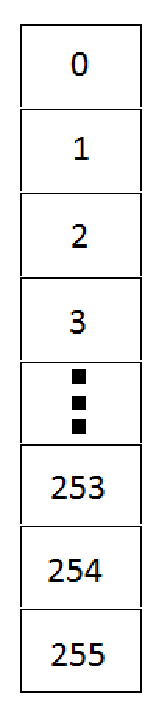
\includegraphics[scale=0.7]{figuras/tabela.eps}
	\caption{Tabela de bytes para uso do algoritmo}
\end{figure}

Como a produção deverá ser totalmente balanceada, há a possibilidade de se produzir um resultado em uma posição na tabela já ocupada, para contornarmos esse problema, propomos a seguinte solução: a introdução da variável \textbf{j}

\begin{figure}[h]
	\centering
	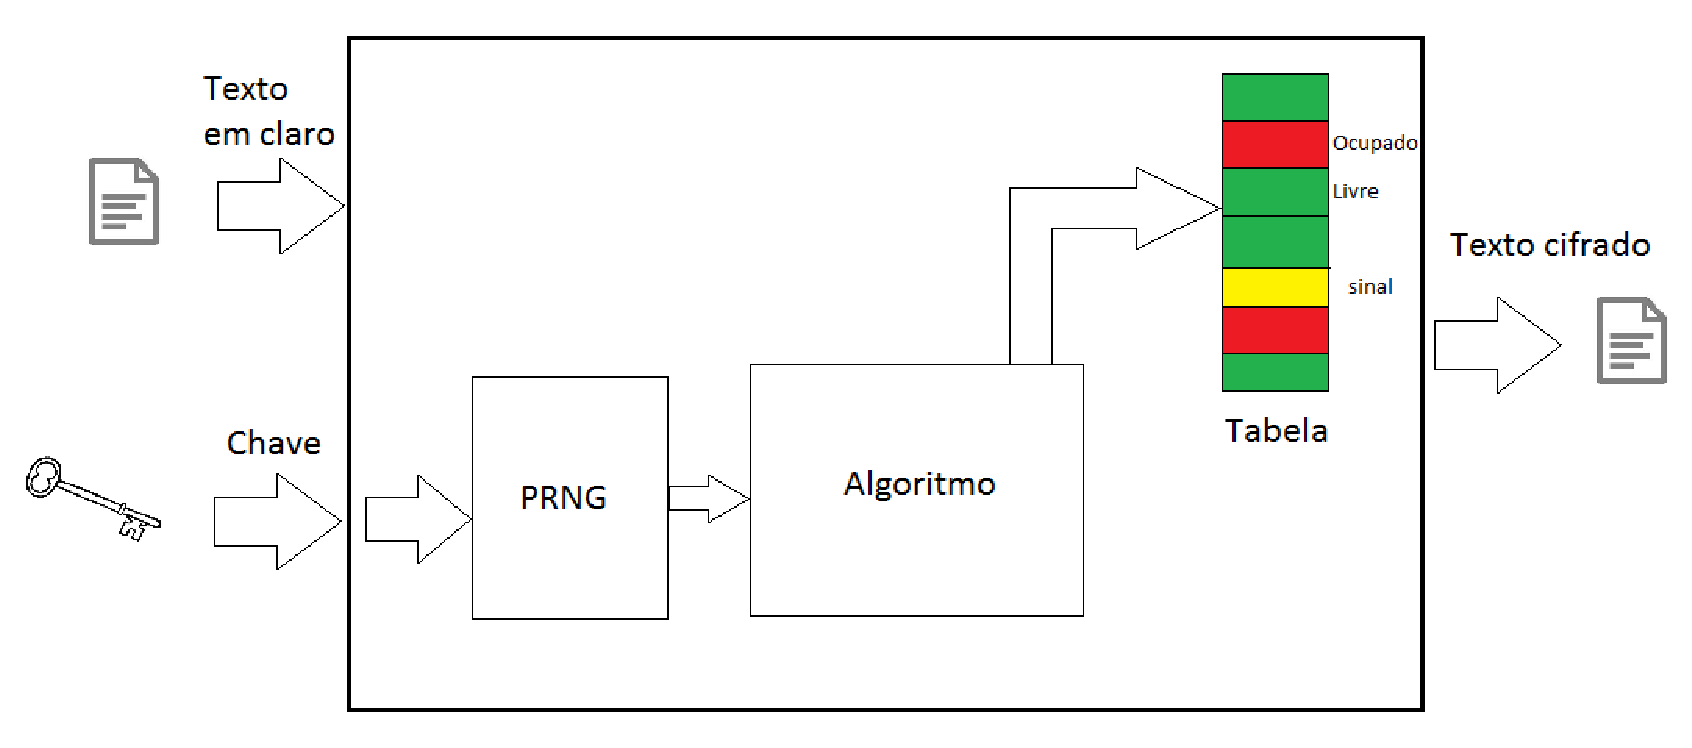
\includegraphics[scale=0.6]{figuras/funcionamento.eps}
	\caption{Esquema do algoritmo}
\end{figure}


\begin{figure}[h]
	\centering
	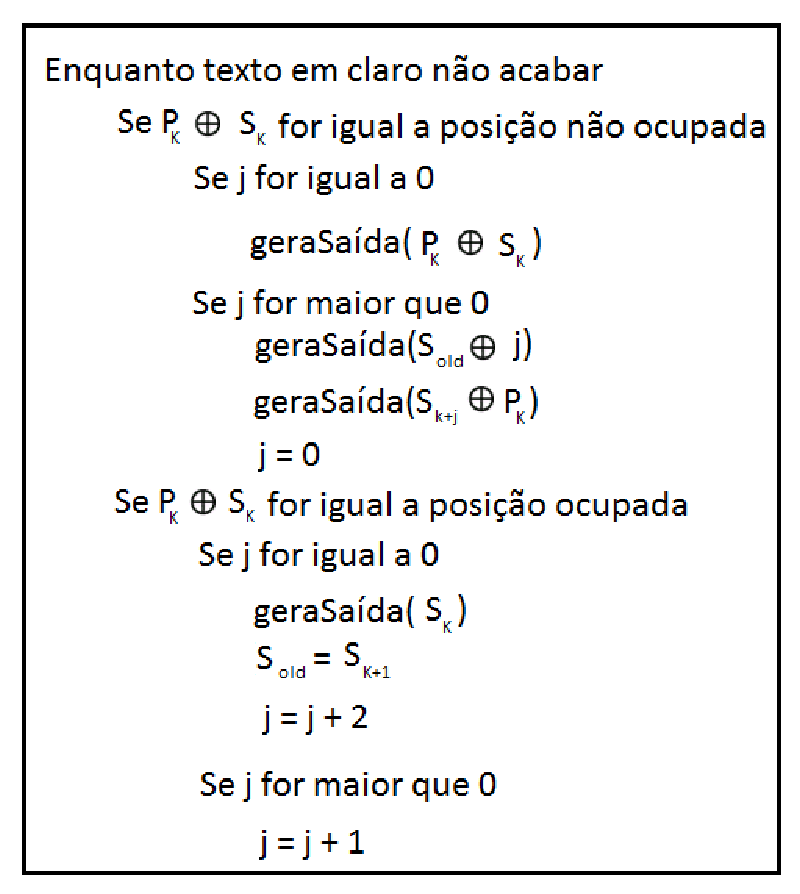
\includegraphics[scale=0.9]{figuras/pseudocondigo.eps}
	\caption{Pseudo código do algoritmo}
\end{figure}

Essa variável visa quantificar os números pseudo-aleatórios que deverão ser descartados na produção do texto cifrado e com isso o receptor da mensagem terá a possibilidade de recuperar a mensagem original com sucesso. Essa solução segue os seguintes passos:

Ou seja, ao se detectar um conflito de resultados na tabela, é enviado o valor S$_k$ para o receptor da mensagem, pois com isso, ao se fazer o ou-exclusivo de S$_k$ com S$_k$ na decifração se obterá o valor 0 e assim o receptor saberá que o próximo valor recebido será a quantidade de números pseudo-aleatórios que deverá ser descartado da sequência. Então o algoritmo vai executar o comando de descartar os números pseudo-aleatórios, até que se encontre um resultado em uma posição que esteja livre. Ao encontrar essa posição livre, o algoritmo deverá enviar o resultado do ou-exclusivo entre j(quantidade de números pulados) e S$_{old}$ e o valor de j é novamente estabelecido como 0.

Quando a tabela for totalmente concluída, o processo se inicia de novo e suas posições ficam livres e o algoritmo continua com o processo de preenche-la novamente. Esse processo só finaliza quando os bytes do texto em claro forem todos cifrados. 

A maior vantagem desse algoritmo é que é muito genérico, ou seja, não importa qual gerador de números pseudo-aleatório será utilizado e também pode-se utilizar em conjunto com outros algoritmos de cifração de fluxo, aumentando a segurança do texto cifrado.